\documentclass[a4paper,12pt]{article}
\usepackage[brazil, english]{babel}
\usepackage[utf8]{inputenc}
\usepackage[T1]{fontenc}
\usepackage{geometry}
\usepackage{setspace}
\usepackage{titlesec}
\usepackage{hyperref}
\usepackage{graphicx}
\usepackage{caption}
\usepackage{subcaption}
\usepackage{fancyhdr}

%%%%%%%%%%%%%%%%%%%%%%%%%%%%%%%%%%%%%%%%%%%%%%%%%%
% These are some new commands that may be useful 
% for paper writing in general. If other new commands
% are needed for your specific paper, please feel 
% free to add here. 
%
% The currently available commands are organized in: 
% 1) Systems
% 2) Quantities
% 3) Energies and units
% 4) particle species
% 5) Colors package
% 6) hyperlink
%%%%%%%%%%%%%%%%%%%%%%%%%%%%%%%%%%%%%%%%%%%%%%%%%%

\usepackage{amsmath}
\usepackage{amssymb}
\usepackage{upgreek}
\usepackage{multirow}
\usepackage{setspace}% http://ctan.org/pkg/setspace
\usepackage{fancyhdr}
\usepackage{datetime}

% 1) SYSTEMS
\newcommand{\btc}               {\textbf{BTC}}
\newcommand{\btcspace}          {\textbf{BTC} }
\newcommand{\pow}               {\textbf{PoW}}

% 4) definition to references, biblatex and hyperlink
\usepackage[backend=bibtex, 
style=nature,  %style reference.
sorting=none,
firstinits=true %first name abbreviate
]{biblatex}

\usepackage{hyperref}
\hypersetup{
    colorlinks=true, %set "true" if you want colored links
    linktoc=all,     %set to "all" if you want both sections and subsections linked
    linkcolor=blue,  %choose some color if you want links to stand out
    citecolor= blue, % color of \cite{} in the text.
    urlcolor  = blue, % color of the link for the paper in references.
}

% 5) Tikz and figures
\usepackage{epsfig}
\usepackage{lmodern}
\usepackage{mathtools}
\usepackage[utf8]{luainputenc}
\usepackage{xspace}
\usepackage{tikz}
\usepackage{pgfplots}
\pgfplotsset{compat=newest}

\usetikzlibrary{positioning}
\usepackage{subcaption}

% 6) colors:
\usepackage{xcolor}
\definecolor{ao(english)}{rgb}{0.0, 0.5, 0.0} % dark green

% 7) Add lines numbers
%\usepackage{lineno}

% add pdf file to thesis:
\usepackage{pdfpages}

\hypersetup{
    colorlinks=true,% make the links colored
    linkcolor=blue
}

\usepackage{setspace}
\addbibresource{bibliography.bib}

\newcommand{\printingbibliography}{%

    \pagestyle{myheadings}
    \markright{}
    \sloppy
    \printbibliography[heading=bibintoc, % add to table of contents
                   title=Refer\^encias % Chapter name
                  ]
    \fussy%
}
\PassOptionsToPackage{table}{xcolor}

\pagestyle{fancy}
\fancyhf{}
\renewcommand{\headrulewidth}{0pt}
\fancyhead[R]{\thepage}

\geometry{a4paper,top=30mm,bottom=20mm,left=30mm,right=20mm}

\titleformat*{\section}{\bfseries\large}
\titleformat*{\subsection}{\bfseries\normalsize}

\title{ \textbf{\large Plano de Aula - F\'isica}}
\author{ANDRÉ VIEIRA DA SILVA}
\date{28 de Maio de 2024}

\begin{document}

\maketitle

%\selectlanguage{brazil}
%
%\begin{abstract}
%\textbf{PALAVRAS CHAVE: }.
%\end{abstract}
%
%\selectlanguage{english}
%\begin{abstract}
%
%\textbf{KEYWORDS: A}.
%\end{abstract}
%
%\selectlanguage{brazil}
%
%\newpage
%\hypersetup{linkcolor=blue}
\tableofcontents
\newpage

\setstretch{1.3} % Altere o valor 1.2 para o valor desejado

\section*{Introdu\c{c}\~ao}
\hspace{0.5cm}Para iniciar os planos de aula para o Ensino de F\'sica,
devemos fornecer o contexto necess\'ario para facilitar a compreens\~ao
do conte\'udo de F\'isica. Aqui ser\~ao escritos 10 planos para os 
seguintes t\'opicos:

\begin{itemize}

    \item 1. \bf{Leis de Newton.}
    \item 2. \bf{Conservação da energia e momentos. }
    \item 3. \bf{Gravitação. }
    \item 4. \bf{Leis da termodinâmica. }
    \item 5. \bf{Óptica física. }
    \item 6. \bf{Oscilações e ondas.} 
    \item 7. \bf{Equações de Maxwell.} 
    \item 8. \bf{Radiação do corpo negro, efeito fotoelétrico e efeito Compton. }
    \item 9. \bf{Relatividade restrita. }
    \item 10. \bf{Decaimentos nucleares e aplicações.}
\end{itemize}

\newpage
\section{Leis de Newton}
\begin{itemize}
\item \textbf{Conte\'udo}: Din\^amica.
\item \textbf{Objetivo}: Compreender as Leis de Newton e como elas explicam a causa
do movimento dos corpos.
\item \textbf{Tempo de Aula}: 40 min.
\end{itemize}




%\begin{figure}[!h]
%    \centering
%    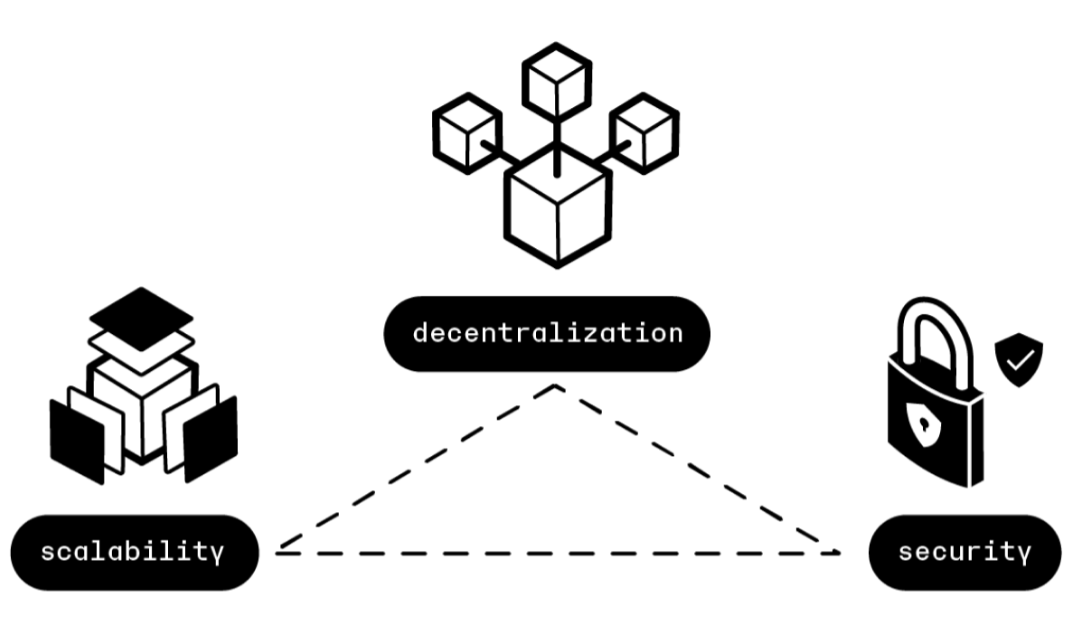
\includegraphics[width=0.8\textwidth]{images/trillemabtc.png}
%    \caption{Trillema das Blockchains. Figura retirada do site \href{https://coinloan.io/blog/what-is-blockchain-trilemma/}{What is Blockchain Trillema}.}
%    \label{trillemablockchain}
%\end{figure}


%%%%%%%% Bibliography 
% Os comandos para incluir as referências bibliográficas
\printingbibliography

\end{document}
